\section{Introduction}

(Motivation) 
Event-series pattern matching is widely used for behavioral/anomaly/causality
analysis, for eg: network diagnostics, algorithmic
trading, security breach detection.


(Challenges)
Warehoused data is being analyzed by a wide range of queries thus it
may not be clustered/sorted on time. 
For example, along with pattern matching queries, one might want to answer also 
queries like in which city are located most of the last month's website 
visitors. 
These queries have very different optimum data layout, and as the latter kind 
are usually much more frequent, their optimum data layout ends up becoming the 
layout of choice in the data center.
Keeping a second copy of the data sorted on time is wasteful in terms of space, 
especially in the light of the fact many of the recorded events are not 
referenced by patterns. 
That is why, before sorting the data and feeding it to a pattern matching 
engine, an extra preprocessing step is used to discard all the events that do 
not satisfy any of the selection predicates of the pattern.     

We also note that the input data is not necessarily sorted on time in the first 
place either, as it may be collected from a wide array of sources, with varying 
constraints for when the data ingestion should happen. 

Analytics are being run both over fresh data as well as historical data,
therefore the data management system needs to support both online and
batching mode processing.


(Approach)
We design a set of relational-style optimizations for event-series pattern
matching workloads.

Relation to abstract interpretation, i.e.\ how abstract filters relax the 
precise constraints enforced by the pattern regarding which events form 
successful matches. 
The relaxation/coarsening is done in a conservative manner, with the guarantee 
that the abstract filter only discards events that would otherwise not take 
part in a complete match. 

(Results)
We provide X reduction in shuffled data and Y reduction in end-to-end latency
for 3 workloads:
i) telemetry analysis over the events produced by the Windows event-reporting
infrastructure
ii) Github queries
iii) stock market algorithmic trading.









\section{Motivating example}

Let us consider an analytics task that mines influential reviews
within the click-stream of an e-commerce website consisting of events of type
``Search''(S), ``Read review''(R) and ``Purchase''(P).
The mining task is described in terms of a pattern initiated by a ``Search''
event, followed by any number of ``Read review'' events and that concludes with
a ``Purchase'' event. 
All events are correlated by the id of the user that performed them and the
``Purchase'' event must occur within a timeout $t_{out}$ from the ``Search'' event. 
The symbolic automata representation of the pattern is given in
figure~\ref{fig:srp_pattern} where we consider as input an Events(name, time,
user) relation with fields for event name, event timestamp and
associated user id, and we use $.$ as a shorthand for the conjunctive operator.

The typical execution plan of this task on a map-reduce framework is to first
group all events by user id, then sort them on time and finally run a pattern
matching engine to detect the desired sequence of events.
In this work we propose to greatly expand the array of possible execution plans
by taking advantage of the fact that a large class of patterns can be
equivalently expressed as SQL queries.
By doing so then one can leverage decades of progress in query optimization to
come up with more efficient query plans than the one outlined above.

For instance, one can express our example pattern as a SQL query as follows:
\begin{verbatim}
SELECT S.user, S.time, P.time
FROM Events S, Events P
WHERE S.name == "S" AND P.name == "P"  
AND   S.time < P.time AND P.time < S.time + t_out
AND   S.user == P.user
AND NOT EXISTS ( 
    SELECT * FROM Events R
    WHERE S.time < R.time AND R.time < P.time
    AND R.user == S.user
    AND R.name != "R"
); 
\end{verbatim}

The first part of the query enforces the fact that a successful match consists
of an event S followed within a timeout $t_{out}$ by an event P from the same user,
while the second part captures the fact that only R events are allowed to take
place in between these two events.
The final result of the query is a set of tuples, one per successful match,
consisting of the user id and the timestamps of the initial and final event
in the match.

Since the number of purchase events P are bound to be much lower than the
search or read review events, performing a broadcast join wrt.\ to the P events
might prove to be the optimum execution plan for this pattern. We remark that
once expressed as an SQL query such optimizations opportunities are dramatically
easier to explore.



The class of patterns that we can currently translate into SQL are those whose
symbolic automata have only cycles of constant length, ie. every repetition
within a particular cycle should consist of the same number of events. 
We note that this class includes the overwhelming majority of patterns discussed
in the literature of complex event processing systems as well as encountered
within an industrial benchmark.

While we acknowledge that for patterns with many transitions, whose
corresponding queries involve many joins, the optimizer might find optimal the
standard query plan based on the pattern matching engine,
we argue that even in such cases one can still leverage the derived query to
minimize the number of events that get grouped by and sorted before being fed to
the pattern matching engine.
Ideally, only the events that will end up as part of a successful match should
undergo this process.
In the following we discuss our approach for performing this pre-filtering step
in a time and space efficient manner, but in order to simplify the presentation
we first re-write the derived query using comprehension syntax.

\begin{align*}
E_S 
&\coloneq 
\{ (t_S, user_S) \mid 
   (n_S, t_S, user_S) \in Events .\ n_S = \text{``S''}
\}
\\
E_{\oR} 
&\coloneq 
\{ (t_{\oR}, user_{\oR}) \mid 
   (n_{\oR}, t_{\oR}, user_{\oR}) \in Events .\ n_{\oR} \neq \text{``R''}
\}
\\
E_P 
&\coloneq 
\{ (t_P, user_P) \mid 
   (n_P, t_P, user_P) \in Events .\ n_P = \text{``P''}
\}
\\
Q 
&\coloneq 
\{ (user_S, t_S, t_P) \mid 
   (t_S, user_S) \in E_S .\ 
   (t_P, user_P) \in E_P .\
\\ 
&\qqqquad\quad
    t_S < t_P < t_S + t_{out} .\ 
	user_P = user_S .\ 
\\
&\qqqquad\quad
	E_{\oR}(t_S..t_P, user_S) = \emptyset  
\}
\\
\end{align*}



\begin{figure}[t]
\centering
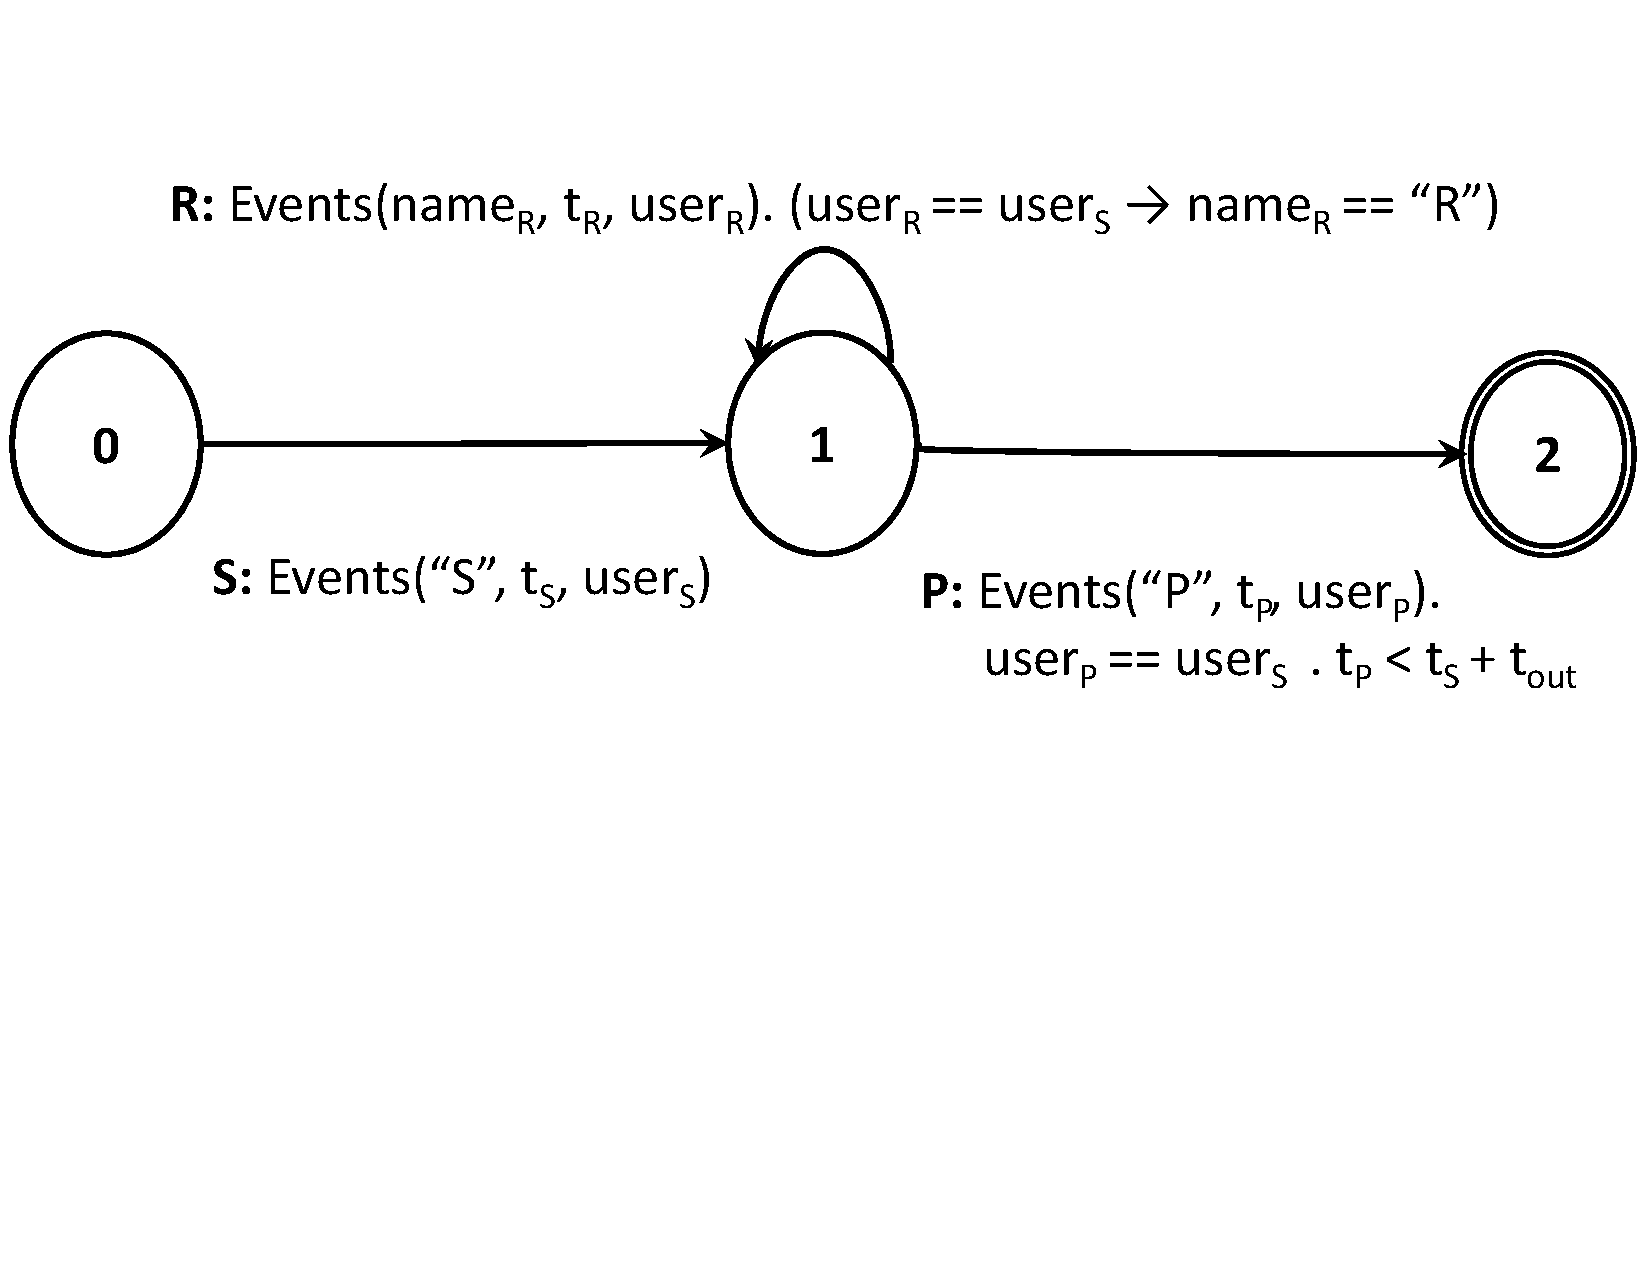
\includegraphics[clip, trim=0.5cm 10cm 0.5cm 3cm,width=\columnwidth]
{graphs/example_sm.pdf}
\caption{Symbolic automata for the SR*P pattern.}
\label{fig:srp_pattern}
\end{figure}

In defining $Q$ we rely on intermediary relations 
$E_S, E_P$, and $E_{\oR}$, representing the set of ``S'' events, ``P'' events
and the complement of the set of ``R'' events, respectively.
Furthermore, we use $E_{\oR}(t_S..t_P, user_S)$ to denote the slicing of
$E_{\oR}$ as follows:
\begin{align*}
\{ (t_{\oR}, user_{\oR}) \mid 
   (t_{\oR}, user_{\oR}) \in E_{\oR} .\ 
   t_S < t_{\oR} < t_P .\ 
   user_{\oR} = user_S
\},
\end{align*}
which we then use in re-writing the \texttt{NOT EXISTS} sub-clause as an
emptiness test.


Towards our goal of removing events from the input that are guaranteed not to
participate in a successful match, and as such minimize the number of events
being sorted and considered by the pattern matcher, we
generate a {\em precise filter} for each transition in the pattern. 
For our example pattern we get the following filters:
\begin{align*}
M_S 
&\coloneq 
\{ (t_S, user_S) \mid 
   (t_S, user_S) \in E_S .\
\\
&\qqqquad 
   \exists\ (t_P, \_) \in E_P(t_S..t_S + t_{out}, user_S) .\ 
\\
&\qqqquad\quad
   E_{\oR}(t_S..t_P, user_S) = \emptyset 
\}
\\
M_R 
&\coloneq 
\{ (n_R, t_R, user_R) \mid 
   \exists (\_, t_S, t_P) \in Q .\ 
\\
&\qqqquad\quad
   (n_R, t_R, user_R) \in Events(*, t_S..t_P, *) 
\}
\\
M_P 
&\coloneq 
\{ (t_P, user_P) \mid  
   (t_P, user_P) \in E_P .\ 
\\
&\qqqquad
   \exists\ (t_S, \_) \in E_S(t_P-t_{out}..t_P, user_P) .\ 
\\
&\qqqquad\quad
   E_{\oR}(t_S..t_P, user_P) = \emptyset 
\}.
\end{align*}

Since evaluating these filters would in many cases be as expensive as computing
the complete result $Q$, we use them only as a starting point for deriving a set
of {\em symbolic filters}, as a ``relaxed'' version of the {\em precise
filters}, but that can be applied with low processing and communication costs.
We do so by employing a series of {\em data and predicate abstractions} 
that generate conservative versions of the original filters.


We showcase our techniques on the filter corresponding to the S transition,
which we first complement in order to obtain the set of events matching
transition S but that will not be part of a complete match.

\newcommand{\oMS}{\overline{M_S}}
\newcommand{\NotExistsP}{\ident{NotExistsP}}
\newcommand{\NotPrecedesP}{\ident{NotPrecP}}

\newcommand{\interval}[1]{\lfloor #1 \rceil}
\newcommand{\uinterval}[1]{\lceil #1 \rfloor}
\newcommand{\hashid}[1]{\langle #1 \rangle}


\begin{align*}
&
\oMS \coloneq 
\{ (t_S, user_S) \mid (t_S, user_S) \in E_S .\ 
   \NotPrecedesP(t_S, user_S) 
\}
\\
&
\NotPrecedesP(t_S, user_S) \coloneq 
\forall\; (t_P, \_) \in E_P(t_S..t_S + t_{out}, user_S) .\ 
\\
&\qqqquad\qquad\quad
E_{\oR}(t_S..t_P, user_S) \neq \emptyset 
\end{align*}

This filter highlights the fact that we can safely remove all ``S'' events that
do not have only ``R'' events between themselves and every succeeding event
``P'' occurring within a $t_{out}$ window of time.

In order to minimize the cost of filtering we use {\em data
abstraction} to compute time and space efficient representations of sets $E_S$
and $E_{\oR}$.
For example, one could choose to abstract over time and coarsen timestamps $t$
into time intervals $\interval{t}$. 
Then, the time dimension of sets $E_S$, $E_{\oR}$ could be efficiently encoded
and queried as interval maps, i.e.\ bit vectors where each bit corresponds to a
time interval and a set bit would denote the fact that an event has occurred
within the corresponding interval.
Using this abstraction the filtering predicate becomes:
\begin{align*}
&
\NotPrecedesP^{\interval{t}}(t_S, user_S) \coloneq 
\forall\; (t_P, \_) \in E_P(\interval{t_S..t_S + t_{out}}, user_S) .\ 
\\
&
\qqqquad\qqquad
E_{\oR}(\uinterval{t_S..t_P}, user_S) \neq \emptyset ,
\end{align*}
where in order to maintain conservativeness (ie.\
$\NotPrecedesP^{\interval{t}} \rightarrow \NotPrecedesP$) we had to
over-approximate the $t_S..t_S + t_{out}$ range but under-approximate the
$t_S..t_P$ interval.
Thus, we note that, depending on the filter, the data abstractions that we
use must be able to provide both over- and under- approximations of the original
sets.

If on the other hand we abstract over user ids via hashing, that is
use a compact representation of sets $E_S$, $E_{\oR}$ that stores time
information only per user hash bucket as opposed to individual user ids, then
the resulting symbolic filter:
\begin{align*}
&
\NotPrecedesP^{\hashid{user}}(t_S, user_S) \coloneq 
\\
&
\forall\; (t_P, \_) \in E_P(t_S..t_S + t_{out}, \hashid{user_S}) .\ 
E_{\oR}(t_S..t_P, \hashid{user_S}) \neq \emptyset ,
\end{align*}
does not satisfy our safety requirement 
(i.e.\ $\NotPrecedesP^{\hashid{user}} \nrightarrow \NotPrecedesP$).
This happens because hashing can only provide over-approximations of sets while,
in order to ensure conservativeness, the abstractions used for this filter need
to provide both over and under approximations.

One way to address this issue is to re-write the precise filter using min
aggregates:
\begin{align*}
&
\NotPrecedesP'(t_S, user_S) \coloneq 
\\
&\qquad
\min \{ t_{\oR} \mid (t_{\oR}, \_) \in E_{\oR}(t_S..t_S + t_{out}, user_S) \}
\\
&\qquad
< \min \{ t_P \mid (t_P, \_) \in E_P(t_S..t_S + t_{out}, user_S) \}.
\end{align*}
Now, we can safely use hashing to abstract over user ids based on the following
symbolic filter:
\begin{align*}
&
\NotPrecedesP'^{\hashid{user}}(t_S, user_S) \coloneq 
\\
&\qquad
\max_{u \in \hashid{user_S}}
\min \{ t_{\oR} \mid (t_{\oR}, \_) \in E_{\oR}(t_S..t_S + t_{out}, u) \}
\\
&\qquad
< 
\min_{u \in \hashid{user_S}}
\min \{ t_P \mid (t_P, \_) \in E_P(t_S..t_S + t_{out}, u) \}.
\end{align*}


While for our example it was possible to come up with an alternative formulation
of the filter, this may not always be the case. 
And even in the cases where it is, the alternatives may be too expensive to
materialize and query (for eg.\ evaluating $\NotPrecedesP'^{\hashid{user}}$ is
clearly more costly than $\NotPrecedesP^{\interval{t}}$).
Consequently, 
we introduce {\em predicate abstraction}, a technique
that strengthens the filter by discarding those predicates that cannot be safely
or efficiently abstracted over.
For instance, our filter could be strengthened into:
\begin{align*}
&
\NotPrecedesP''(t_S, user_S) \coloneq 
E_P(t_S..t_S + t_{out}, user_S) = \emptyset,
\end{align*} 
which eliminates only those search events that are not followed by a purchase
event within $t_{out}$, and was obtained from the base case of
the universal quantifier in $\NotPrecedesP$.
Since this version only requires over-approximation, one can safely use hashing
to abstract over the user id dimension of $E_P$, i.e.\ 
$\NotPrecedesP''^{\hashid{user}} \rightarrow \NotPrecedesP''$, where
\begin{align*}
&
\NotPrecedesP''^{\hashid{user}}(t_S, user_S) \coloneq 
E_P(t_S..t_S + t_{out}, \hashid{user_S}) = \emptyset .
\end{align*}

Moreover, predicate abstraction also reveals the well known Bloom
join algorithm as an instance of our approach, wrt.\ the join
predicate $user_P = user_S$ from the original query. 
This becomes apparent if we ignore time in the filter above:
\begin{align*}
&
\NotPrecedesP'''^{\hashid{user}}(t_S, user_S) \coloneq 
E_P(*, \hashid{user_S}) = \emptyset,
\end{align*}
and we use a bloomfilter to implement $E_P(*, \hashid{user_S})$.

A detailed discussion of other scenarios where predicate abstraction proves
beneficial can be found in section~\ref{sec:pred_abstraction}.




\begin{comment}
\\
&
\NotExistsP(t_S, user_S) \coloneq 
E_P(t_S..t_S+t_{out}, user_S) = \emptyset

These filters are designed to be applied independently over the input without
the need to perform any joins, group by's or order by's.
More importantly, in a map-reduce framework they can be performed with minimal
communication overhead.


- interval map may use different granularities in different regions of the
timeline, i.e. finer granularity in regions with higher probability of events
\end{comment}


















